\documentclass{article}
\usepackage{graphicx}
\usepackage[utf8]{inputenc}
\usepackage[T1]{fontenc}
\usepackage[francais]{babel}
\usepackage{layout}


\begin{document}
\begin{titlepage}
\begin{center}
\Huge Documentation

\normalsize
\vspace{0.5cm}
\Large {\underline{ Groupe 3 Bleu : Sokoban} }

\vspace{1cm}
\normalsize
Goron Nathan, De La Rosa Louis-David, Basset Emilien, Demé Quentin
\newline
\newline

\Huge Algorithme A*, fonctionnement

\end{center}
\end{titlepage}


\newpage
\section{Principes de fonctionnement.}
\subsection{Présentation et objectif:}
L'algorithme A* est un algorithme souvent utilisé pour trouver des chemins dans la résolution de jeux. Il est dans notre cas implémenté sur une grille de Sokoban. En dehors du sokoban où cela nous importe peu, il peut être interrompue pendant son utilisation est relancé plus tard. C'est un algorithme de type "anytime".
Le but de A* est de trouver le chemin \textit{le plus court} pour aller d'un point de départ, à un point d'arrivé. Pour cela l'algorithme garde une liste de toutes les étapes futurs que l'on appel "liste ouverte". Cette liste est établis par la fonction g(n). Ensuite, il choisit parmis cette liste une étape futur qui soit "à priori" la meilleure pour nous mener à l'objectif en un temps qui soit le plus court possible. Pour que cela puisse se faire, nous avons besoin d'une heuristique qui puisse nous aider à déterminer quelle est "à priori" la meilleure option. Une fois que cette option est choisis, l'algorithme passe à la "liste fermé". 
\section{Explication détaillée avec exemples.}
\subsection{Fonctions g et h:}
A chaque étape de l'algorithme, les fonctions g(n) et h(n) sont exécutées pour n étant un point d'arrivé. Cela nous donne les informations suivantes.
\begin{itemize}
\item[• g(n) = Le nombre d'étapes pour aller du point de départ à l'arrivée n.]
\item[• h(n) = L'heuristique qui estime le coup pour aller de n à l'objectif final.]
\item[• f(n) = g(n) + h(n): Le nombre minimum d'étapes si on choisit le point n.]
\end{itemize}
\subsection{Etapes détaillées de l'algorithme:}
Voici les étapes de l'algorithme en langage algorithmique: \newline
Soient: OPEN la liste ouvert \newline
(La partie si dessous n'a pas pu être indentée correctement, attention donc!)
Ajouter DEPART à OPEN \newline
Tant que OPEN n'est pas vide:\newline
	Choisir le N ayant le plus petit f(n)\newline
	Si N est l'objectif alors PASS\newline
	Déplacer N dans CLOSED\newline
	Pour chaque N' = PeuBouger(N, direction):\newline
		g(N')=g(N)+1\newline
		h(N')\newline
		Si N' dans OPEN et nouveau N' n'est pas mieux, CONTINUE\newline
		Si N' dans CLOSED and nouveau N' n'est pas mieux, CONTINUE\newline
		supprimer tout N' étant dans OPEN et CLOSED (en même temps)\newline
		Ajouter N comme parent de N'\newline
		Ajouter N' à OPEN\newline
	FIN POUR\newline
FIN TANT QUE\newline
\textit{Si on arrive ici, alors il n'y a pas de solutions.}
			
\section{Le cas du Sokoban:}
\subsection{Cas général:}
Dans le cas du sokoban, l'heuristique sera le minimum  de déplacements pour atteindre l'objectif si un chemin direct est possible. Or puisque l'on se déplace uniquemment à la verticale ou à l'horizontale, cette donnée sera la somme des déplacements horizontaux et verticaux à réaliser.
\begin{center}
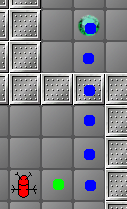
\includegraphics[scale=1]{images/heuristic.png} \newline
\textit{Ce shéma présente le minimum de déplacements pour aller du point rouge au point d'arrivé.}
\end{center}
Ainsi pour l'étape en vert:
\begin{itemize}
\item[g(n)= 1]
\item[h(n)= 6]
\item[f(n)= 1+6 = 7]
\end{itemize}



\newpage
\end{document}